\subsection{API}
	La componente \textit{API} è il core dell'intera architettura; permette all'applicazione web di interfacciarsi con i due database menzionati precedentemente, oltre che con un bot Telegram.
	\newline
	La componente è stata sviluppata in Java 11, utilizzando dei framework Spring: Spring boot, Spring security, Spring kafka e Spring jpa; per l'autenticazione web è stato usato Json Web Token.

	\subsubsection{Diagramma dei package}%%%%%%%%%%%%%%OK
		\begin{figure}[H]
			\centering
			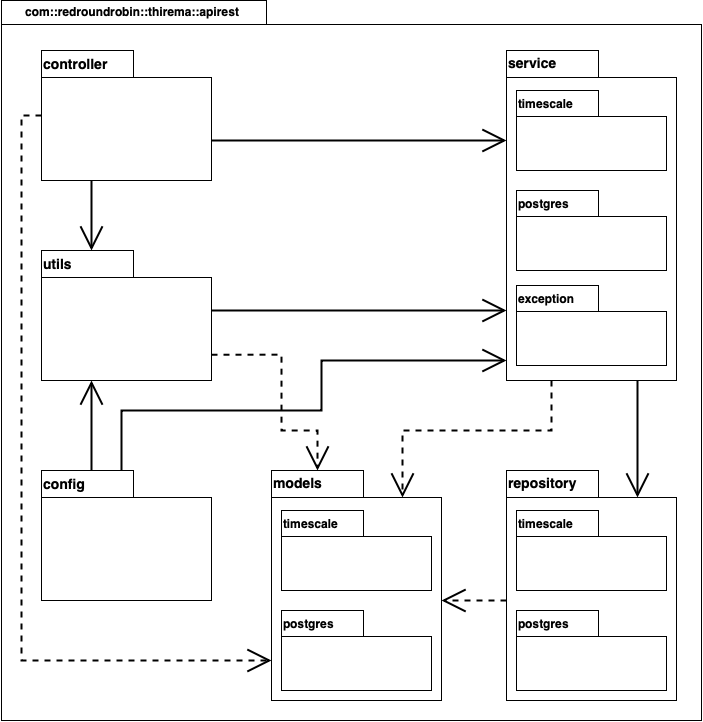
\includegraphics[scale=0.500]{res/images/API/packageAPI.png}
			\caption{Diagramma dei packages per la componente API}
			\label{Diagramma 10}
		\end{figure}

	\subsubsection{Dipendenze esterne}
		La componente \textit{API} he le seguenti dipendenze esterne:
		\begin{itemize}
			\item \textbf{Spring Boot:} che viene utilizzato per rendere le API un microservizio; 
			\item \textbf{Spring Boot Jpa:} contenuta nel framework precedente, viene utilizzata per permettere al package Repository e Config di interfacciarsi direttamente con il database;
			\item \textbf{Spring Boot Starter Security:} contenuta nel framework Spring Boot, viene utilizzata per gestire la sicurezza nell'accesso alle API;
			\item \textbf{SpringBoot Starter Test:} contenuta nel framework Spring Boot, viene utilizzata per eseguire i test;
			\item \textbf{org.Moquito:} libreria usata per fare simulare il comportamento di alcune funzioni, in fase di test;
			\item \textbf{io.jsonwebtoken:} libreria usata per la creazione di token necessari all'accesso ad aree riservate delle API;
			\item \textbf{Spring Kafka:} libreria utilizzata per la comunicazione con Kafka;
			\item \textbf{Spring Doc:} libreria utilizzata per la visualizzazione delle richieste API tramite interfaccia web;
			\item \textbf{org.postgreSql.Driver:} che viene utilizzato per la connessione con DBMS di tipo Postgre.
		\end{itemize}

	\subsubsection{Diagrammi delle classi}
		Al fine di semplificare la comprensione delle dipendenze della componente API, si è deciso di suddividere i diagrammi per package, mostrando in dettaglio quelli più significativi.

		\paragraph*{Package Utils}		
		\begin{figure}[H]
			\centering
			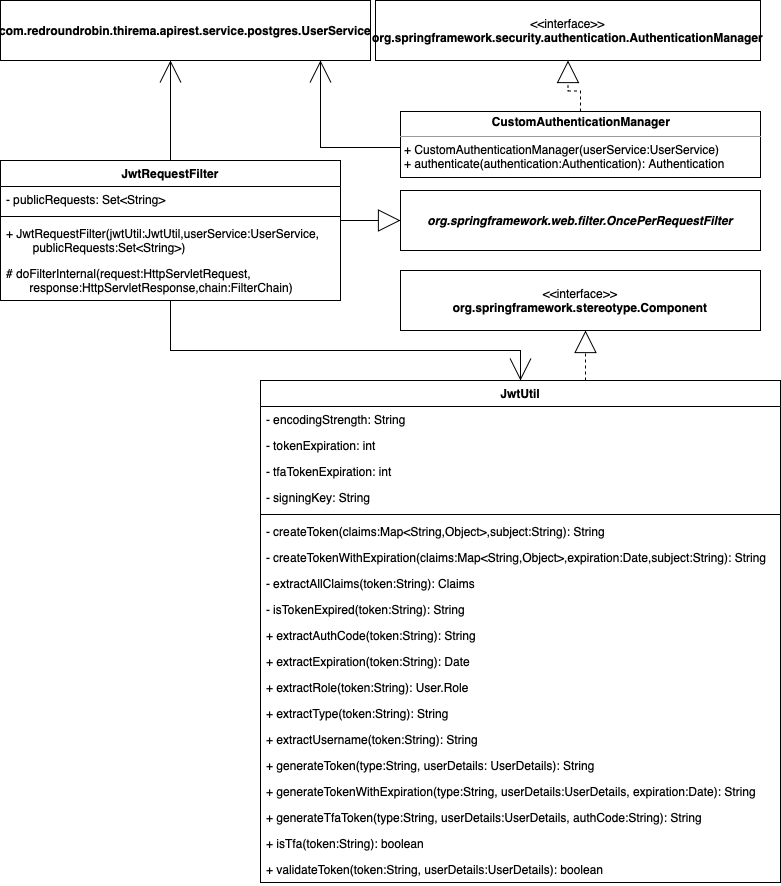
\includegraphics[scale=0.550]{res/images/API/UtilsPackage.png}
			\caption{Diagramma del package utils della componente API}
			\label{Diagramma 11}
		\end{figure}
		Come si evince dal diagramma, la classe JwtRequestFilter dipende dalle classi UserService e JwtUtils ed estende la classe OncePerRequestFilter, permettendo di filtrare le richieste alle API. JwtUtil invece implementa l'interfaccia Component del framework spring. Infine la classe CustomAuthenticationManager dipende da UserService ed implementa l'interfaccia AuthenticationManager del framework Spring, permettendo quindi di gestire l'autenticazione in maniera sicura.
		\paragraph*{Package Config} 
		\begin{figure}[H]
			\centering
			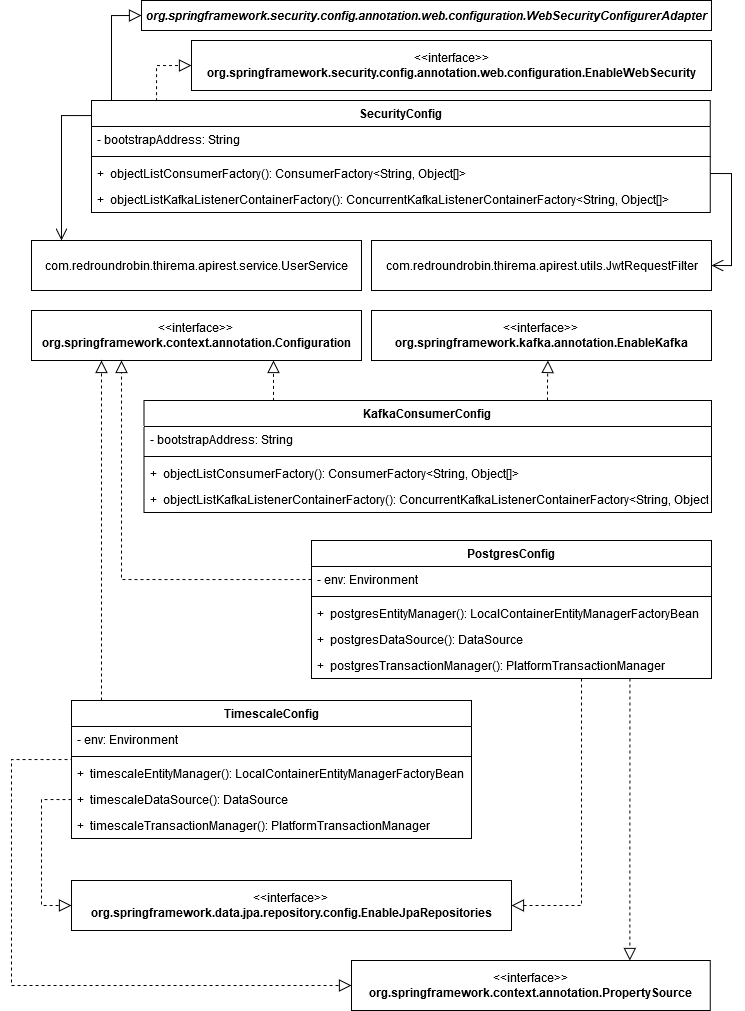
\includegraphics[scale=0.550]{res/images/API/ConfigPackage.png}
			\caption{Diagramma del package config della componente API}
			\label{Diagramma 12}
		\end{figure}
		Il diagramma del package Config mostra le dipendenze delle classi di configurazione della componente API.  PostgresConfig e TimescaleConfig vengono utilizzate per configurare l'accesso ai nostri database ed implementano le interfacce PropertySource, JpaRepository e Configuration del framework Spring. La classe KafkaConsumerConfig invece implementa le interfacce EnableKafka e Configuration del framework Spring per poter collgarsi con il nostro broker Kafka. Infine SecurityConfig dipende dalle classi ed interfacce restanti per permettere la configurazione della sicurezza per permettere o meno ad alcune richieste HTTP di accedere alla API.
		\newpage
		\paragraph{Package Controllers}
		Il package Controllers visualizzabile all'interno del file \textit{Immagini/API-PackageController.png} contiene i controller per mappare le richieste GET e POST che è possibile ricevere da parte della web app o di Telegram. Ogni classe per poter funzionare implementa l'interfaccia RequestMapping e RestController del framework Spring. La classe AuthContoller a differenza delle altre possiede anche delle dipendenze verso CustomAuthenticationManager TelegramService per permettere l'autenticazione a due fattori tramite Telegram.
		\paragraph*{Package Models}
		\begin{figure}[H]
			\centering
			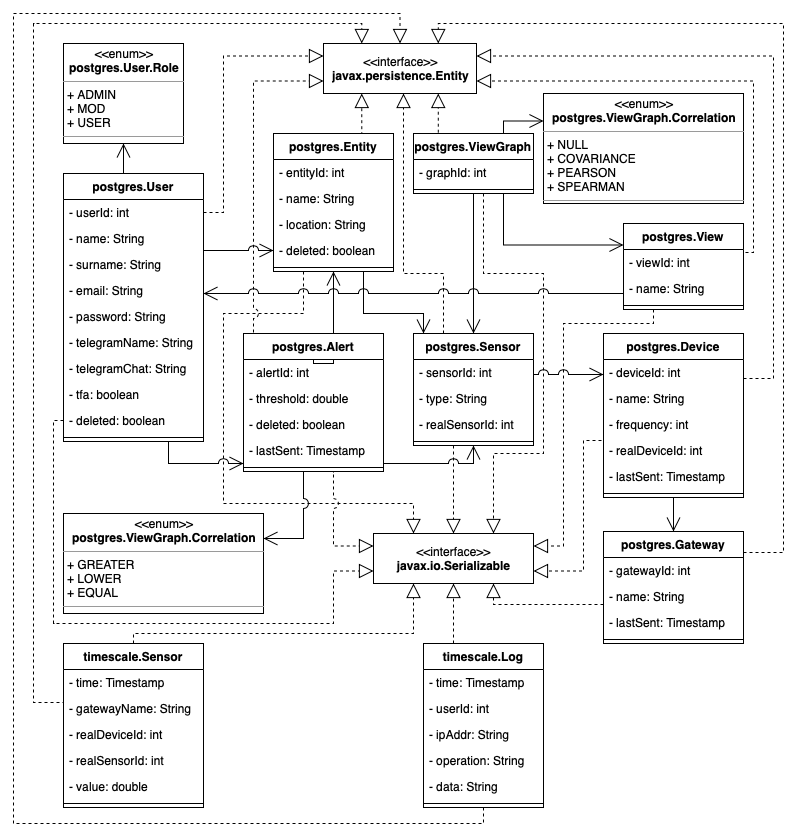
\includegraphics[scale=0.550]{res/images/API/ModelsPackage.png}
			\caption{Diagramma del package models della componente API}
			\label{Diagramma 14}
		\end{figure}
		Nel diagramma in alto vengono descritte le dipendenze del package Models, che rappresentano le relazioni che ci sono fra le varie entità del database relazionale. 
		\begin{landscape}
		\paragraph*{Package Repository}
		\begin{figure}[H]
			\centering
			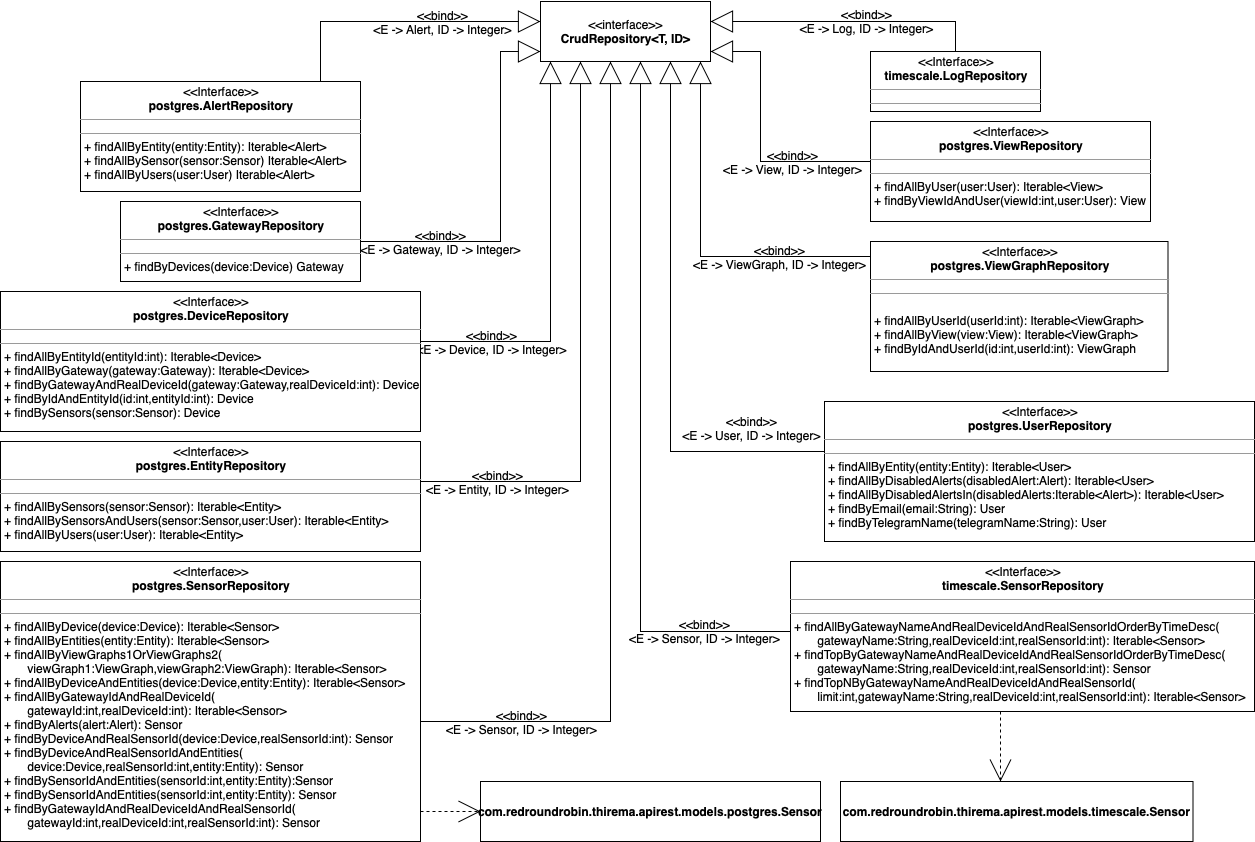
\includegraphics[scale=0.500]{res/images/API/RepositoryPackage.png}
			\caption{Diagramma del package repository della componente API}
			\label{Diagramma 15}
		\end{figure}
		Nel diagramma che rappresenta le dipendenze del package Repository della componente API, sono presenti le interfacce che rappresentano le query che vengono effettuate a database nelle varie tabelle. Tutte le interfacce estendono l'interfaccia CrudRepository.
		\paragraph*{Package Service}
		Nel diagramma delle classi all'interno del file \textit{Immagini/API-PackageService.png} che rappresenta il package Service sono rappresentate classi che effettuano le query a database ad un livello di astrazione più alto rispetto al package Repository. Quest'ultimo viene infatti utilizzato dai service per effettuare le quesry a database.
	
	\subsubsection{Diagrammi di sequenza}%%%%%%%%%OK
		\begin{figure}[H]
			\centering
			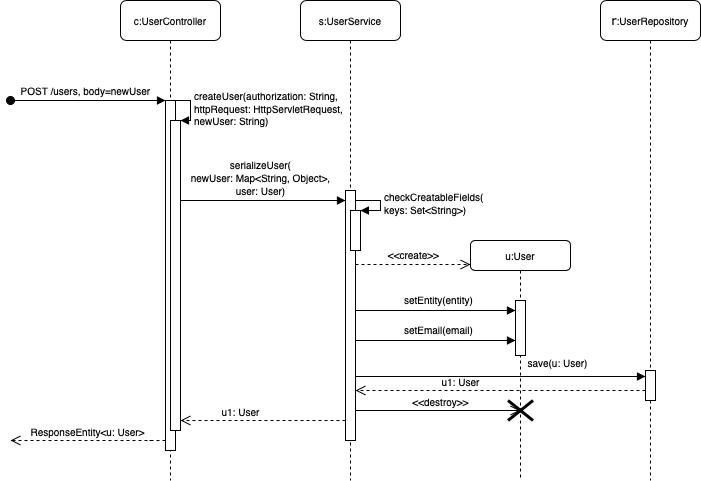
\includegraphics[scale=0.600]{res/images/API/inserimento_utente.png}
			\caption{Diagramma di sequenza che mostra l'inserimento di un utente all'interno della componente API}
			\label{Diagramma 17}
		\end{figure}
		Nel diagramma di sequenza in alto, alla ricezione di una richiesta POST dalla web app, lo UserController chiede allo UserService di inserire un nuovo utente, dopo aver verificato che la richiesta provenisse da un utente con l'autorizzazione necessaria a crearne uno nuovo. Viene creata poi un'istanza di User che, dopo averne impostato i campi, viene inviata a UserRepository, chiedendone il salvataggio nel database. Viene infine restituita l'entità inserita ed inviata in risposta alla web app in formato JSON.
		\begin{figure}[H]
			\centering
			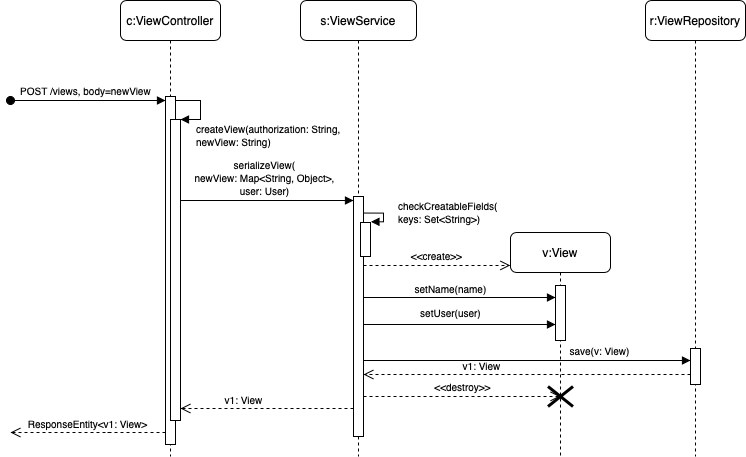
\includegraphics[scale=0.600]{res/images/API/inserimento_view.png}
			\caption{Diagramma di sequenza che mostra l'inserimento di una view all'interno della componente API}
			\label{Diagramma 18}
		\end{figure}
		Il diagramma descrive l'inserimento di una view all'interno del database. Il procedimento inserito è molto simile a quello descritto per l'inserimento di un utente.
	\end{landscape}
	

	\subsubsection{Estensione}
		\paragraph{Aggiungere una richiesta API}
			Per inserire una nuova richiesta, se non si usano le classi già esistenti, è necessario che la nuova classe creata implementi l'interfaccia RestController, tramite la notazione \textit{@RestController}, da inserire precedentemente alla definizione della classe.
			All'interno della classe è necessario definire una funzione usando una notazione di tipo mapping, ad esempio "@GetMapping", inserendo all'interno delle parentesi tonde la stringa associata all'URI della richiesta che si vuole implementare.
			Ad esempio:
			\begin{verbatim}
			@GetMapping(value = \{"/{deviceId:.+}/sensors"\})
			\end{verbatim}
			Per esporre una risorsa senza necessità di autenticazione è necessario aggiungere all'array publicRequests l'URL della richiesta. L'array publicRequests è un attributo della classe SecurityConfig.